
\documentclass[fleqn,addpoints]{exam}

\usepackage{graphicx}
\usepackage{booktabs}
\usepackage{float}
\usepackage{amsmath}
\usepackage{cancel}
\usepackage{polynom}
\usepackage{caption}
\usepackage{mdwlist}

\newcommand{\degree}{\ensuremath{^\circ}} 

\printanswers

\ifprintanswers 
\usepackage{2in1, lscape} 
\fi

\title{Math 115 \\ Homework 29}
\date{July 12, 2011} 

\begin{document}

\maketitle

% \begin{figure}[H]
%   \centering
%   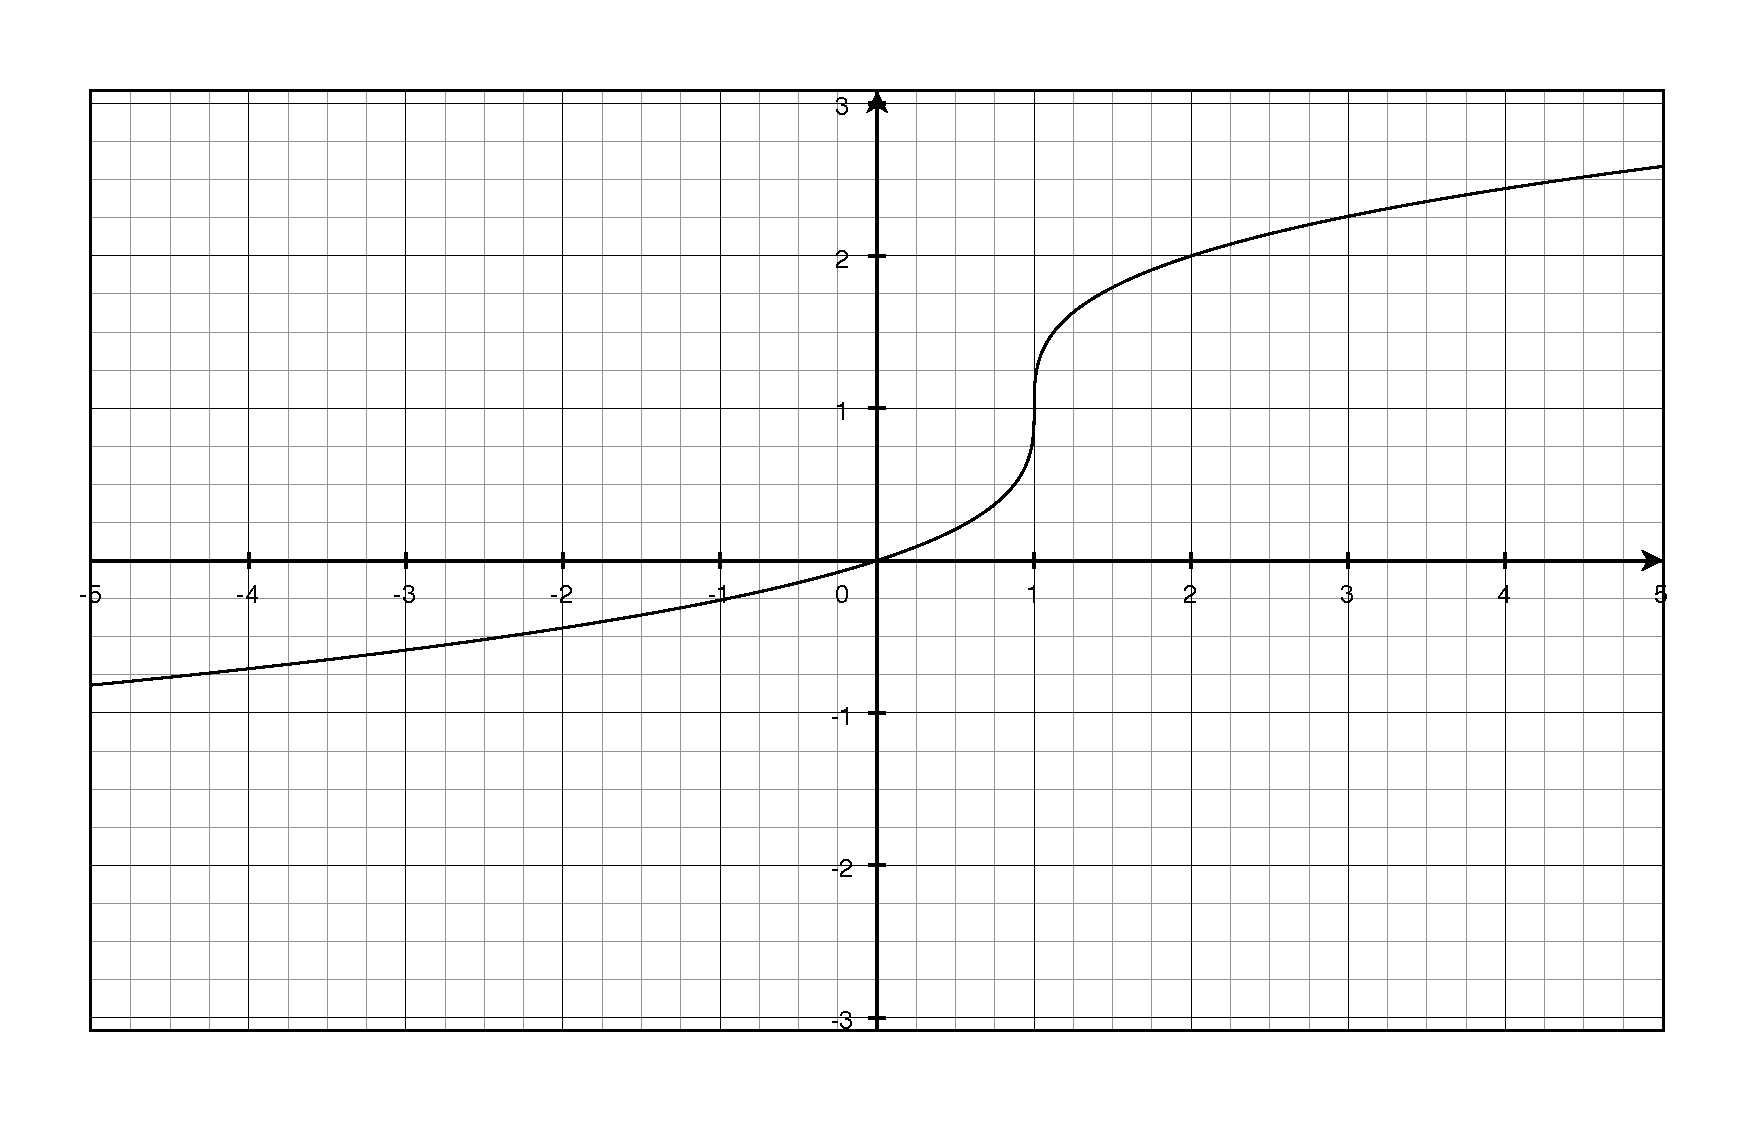
\includegraphics[scale=.3]{question7.eps}
%   \caption*{Question 7}
% \end{figure}

% \begin{tabular}{cc}
% \toprule
% period & amplitude \\
% \midrule
%   $\pi$ & $2$ \\
% \bottomrule
% \end{tabular}

\section{Homework}
\begin{itemize*}
  \item pp. 792-794: 1-7, 11-12, 18-19, 27, 29, 31, 33-34, 41, 43, 47, 51-52
  \item pp. 802-803: 1-4, 7, 9-10, 13-14, 21, 23, 25, 27, 31, 35, 42-49
\end{itemize*}

\section{Extra Credit}
\begin{itemize*}
\item Page 794, question 55
\item Page 803, question 40
\end{itemize*}

\ifprintanswers

\pagebreak

\begin{description}

\item[p 794, question 55]

If we let $r$ be the half the length of a {\em latus rectum}, the distance from one of the points on both the {\em latus
  rectum} and the ellipse to the two foci is: $\sqrt{(2c)^2 + r^2} + r$.  

So:
\begin{align*}
  \sqrt{(2c)^2 + r^2} + r &= 2a \\
  \sqrt{4c^2 + r^2} &= 2a - r \\
  4c^2 + r^2 &= 4a^2 -4ar + r^2 \\
  4c^2  &= 4a^2 -4ar  \\
  c^2  &= a^2 - ar  \\
  r &= \frac{c^2 - a^2}{a} \\
  r &= \frac{b^2}{a} \\
\end{align*}

The length of the {\em latus rectum} is $2r$ or $\dfrac{2b^2}{a}$.

\item[p 803, question 40]

The distance between the pulses is:
\[
  d = 0.001 \text{ s} \cdot 186000 \text{ m/s} = 186 \text{ m}
\]

This is $2a$, so $a=93$ and $b^2 = c^2 - a^2 = 150^2 - 93^2 = 13851$.

The equation of the hyperbola is:
\[
  \frac{x^2}{8649} - \frac{y^2}{13851} = 1
\]

We know the y-coordinate of the ship is 75, so we can plug that in to the equation and figure out what the x coordinate
is: 

\begin{align*}
  \frac{x^2}{8649} - \frac{75^2}{13851} &= 1 \\
  x &\approx 110 \\
\end{align*}

So the ship is at: $(110, 75)$

% check:
% \[
%   \frac{110^2}{8649} - \frac{75^2}{13851} \approx 1
% \]

\section{Pages 792-794}

\item[1] b
\item[2] c
\item[3] d
\item[4] f
\item[5] a
\item[6] e

\item[7]

\begin{tabular}{cccc}
\toprule
center & vertices & foci & eccentricity \\
\midrule
  $(0, 0)$ & $(\pm 5, 0)$ & $(\pm 3, 0)$ & $\dfrac{3}{5}$ \\
\bottomrule
\end{tabular}

\begin{figure}[H]
  \centering
  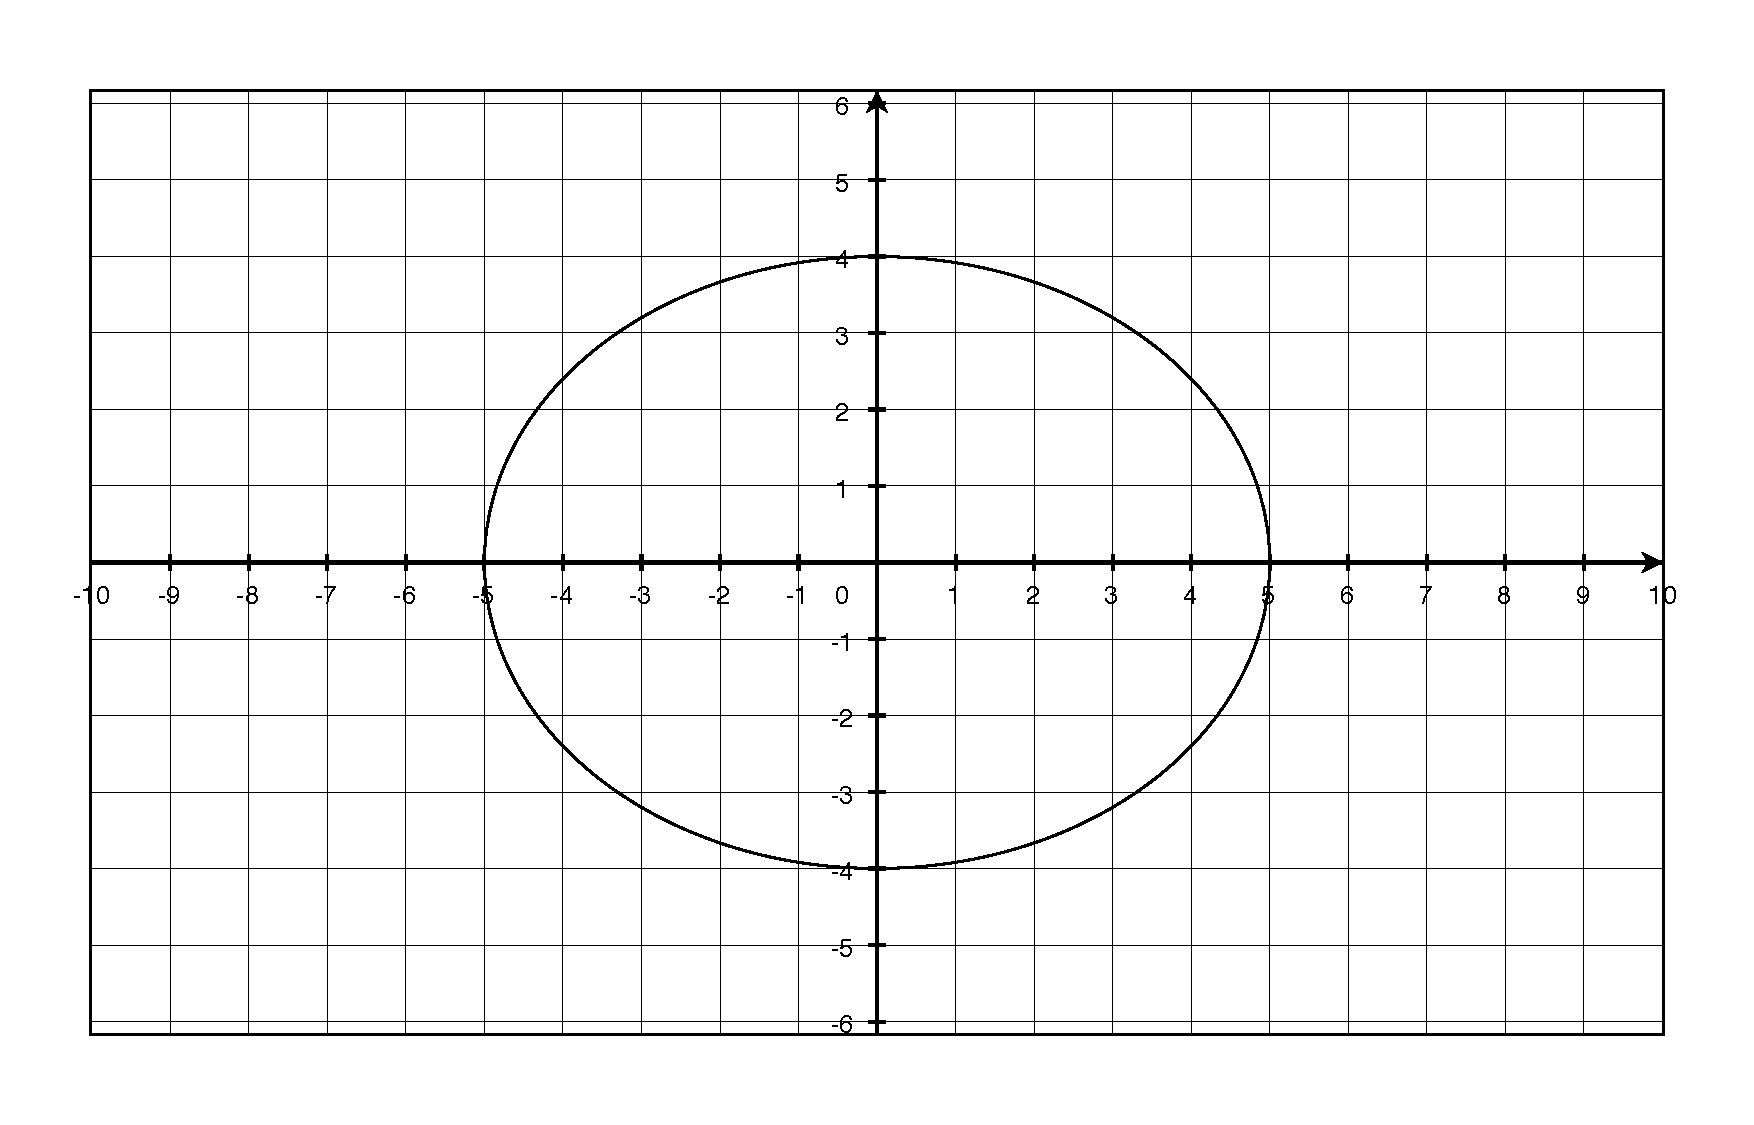
\includegraphics[scale=.3]{p792_7.eps}
  \caption*{Question 7}
\end{figure}

\item[11]

\begin{tabular}{cccc}
\toprule
center & vertices & foci & eccentricity \\
\midrule
  $(-3, 5)$ & $(-3, 10)$, $(-3, 0)$ & $(-3, 8)$, $(-3, 2)$ & $\dfrac{3}{5}$ \\
\bottomrule
\end{tabular}

\begin{figure}[H]
  \centering
  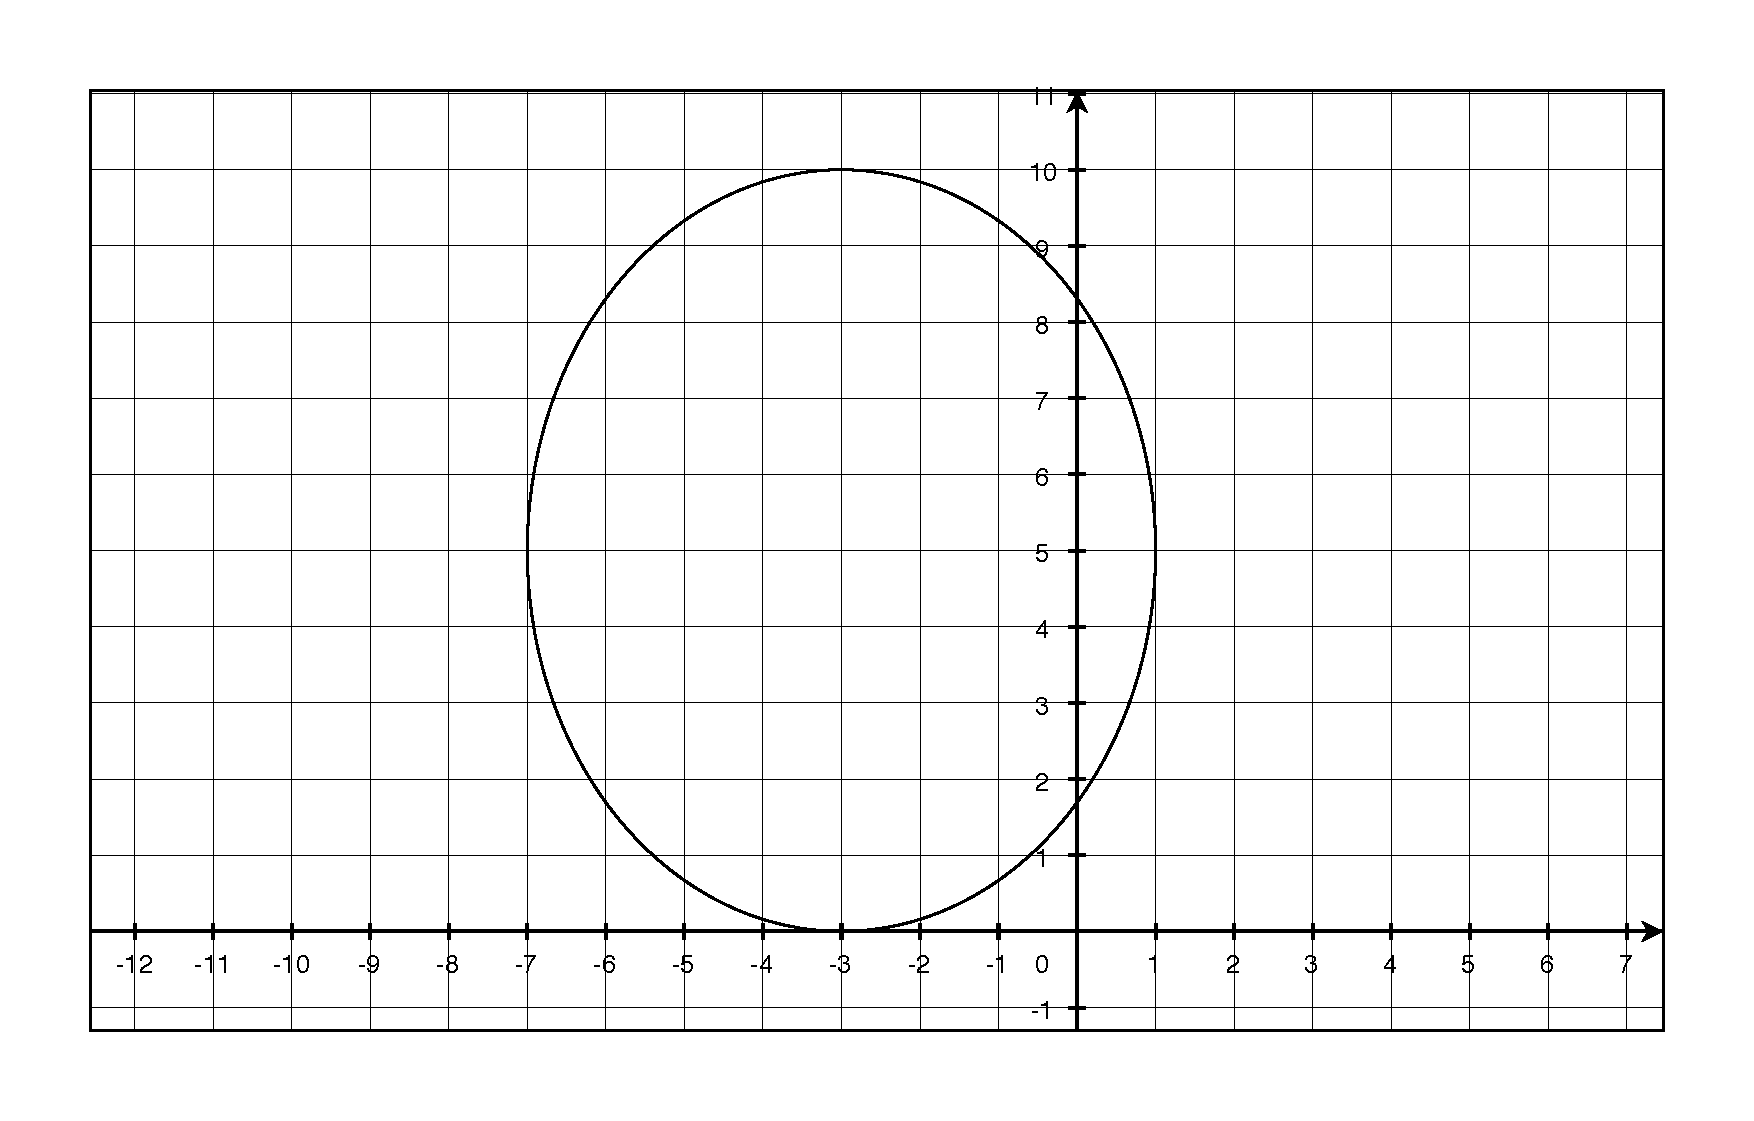
\includegraphics[scale=.3]{p792_11.eps}
  \caption*{Question 11}
\end{figure}

\item[12]
\begin{tabular}{cccc}
\toprule
center & vertices & foci & eccentricity \\
\midrule
  $(4, -3)$ & $(4, 1)$, $(4, -7)$ & $(4, 3)$, $(4, -5)$ & $\dfrac{1}{2}$ \\
\bottomrule
\end{tabular}

\begin{figure}[H]
  \centering
  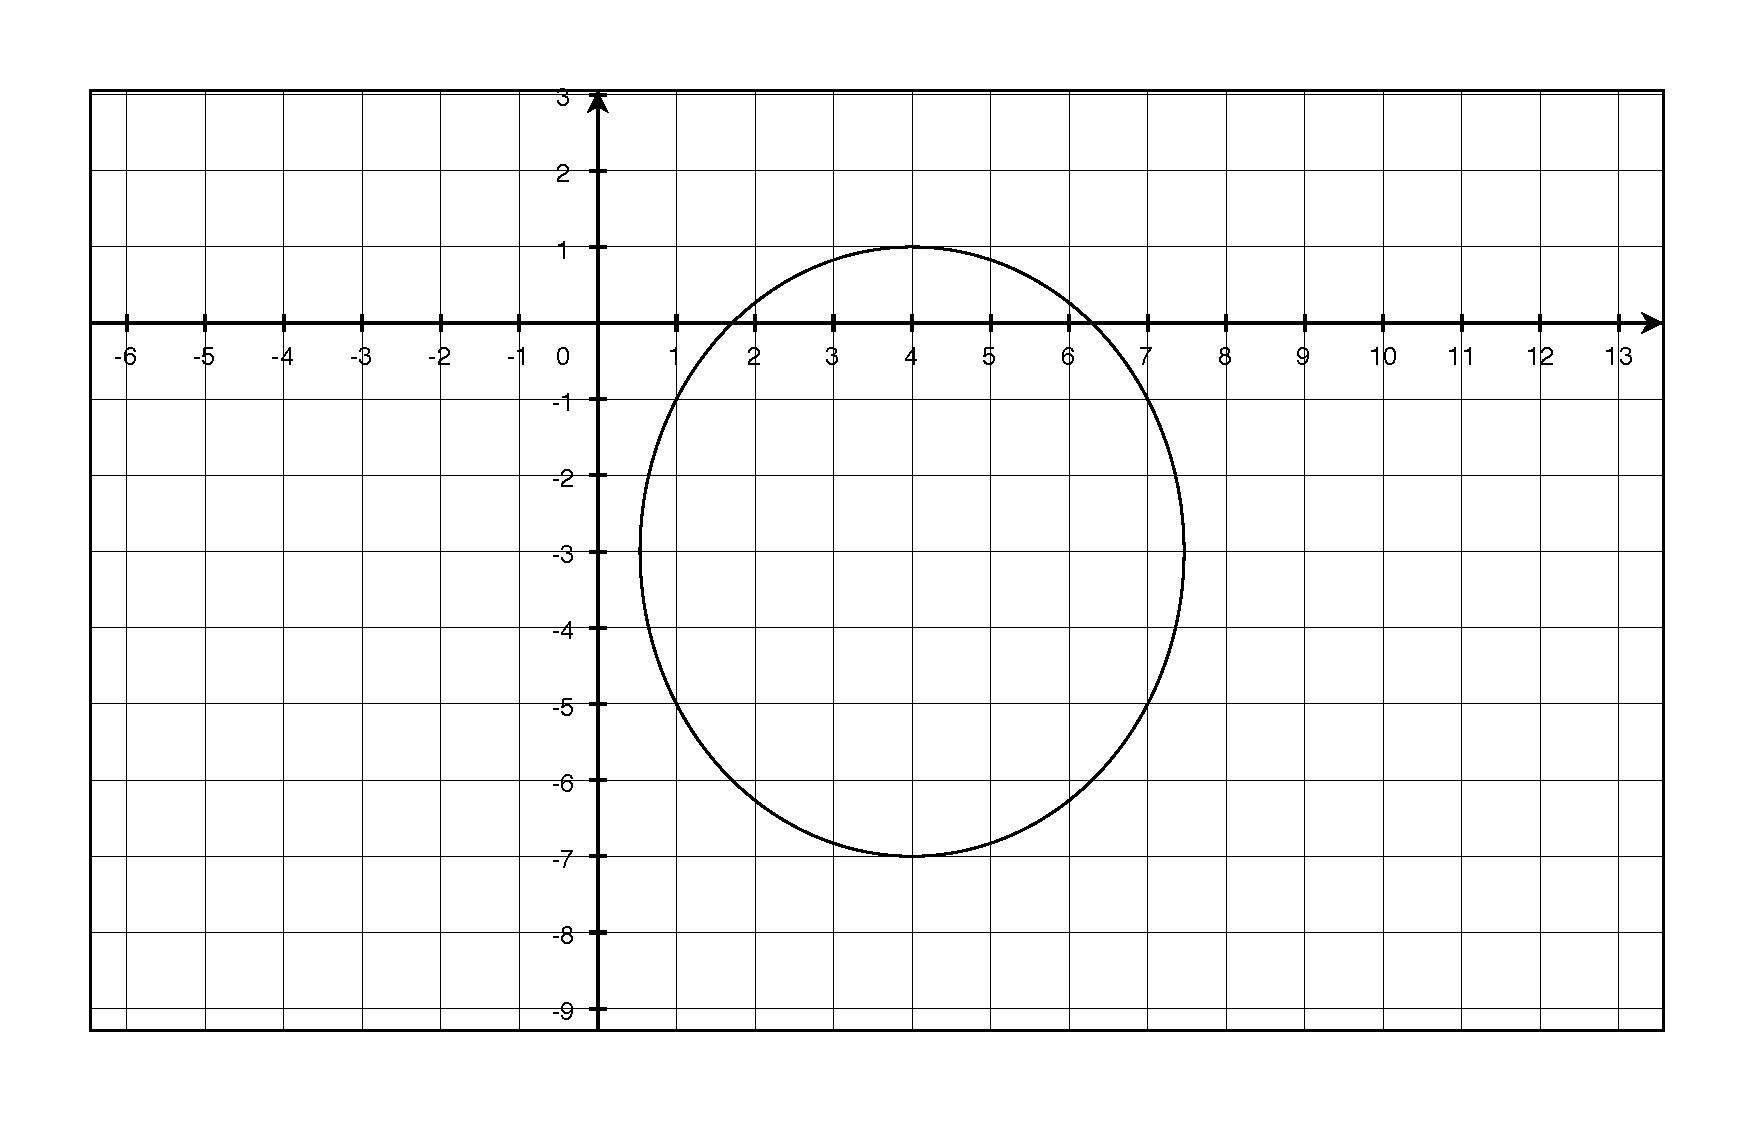
\includegraphics[scale=.3]{p792_12.eps}
  \caption*{Question 12}
\end{figure}

\item[18]
\begin{align*}
  3x^2 + y^2 + 18x - 2y - 8 &= 0 \\
  3(x^2 + 6x + 9) + (y^2 - 2y + 1) &= 8 + 1 + 27 \\
  \frac{(x+3)^2}{12} + \frac{(y-1)^2}{36} &= 1 \\
\end{align*}

\begin{tabular}{cccc}
\toprule
center & vertices & foci & eccentricity \\
\midrule
  $(-3, 1)$ & $(-3, 7)$, $(-3, -5)$ & $(-3, 1 \pm 2\sqrt{6})$ & $\dfrac{\sqrt{6}}{3}$ \\
\bottomrule
\end{tabular}

\begin{figure}[H]
  \centering
  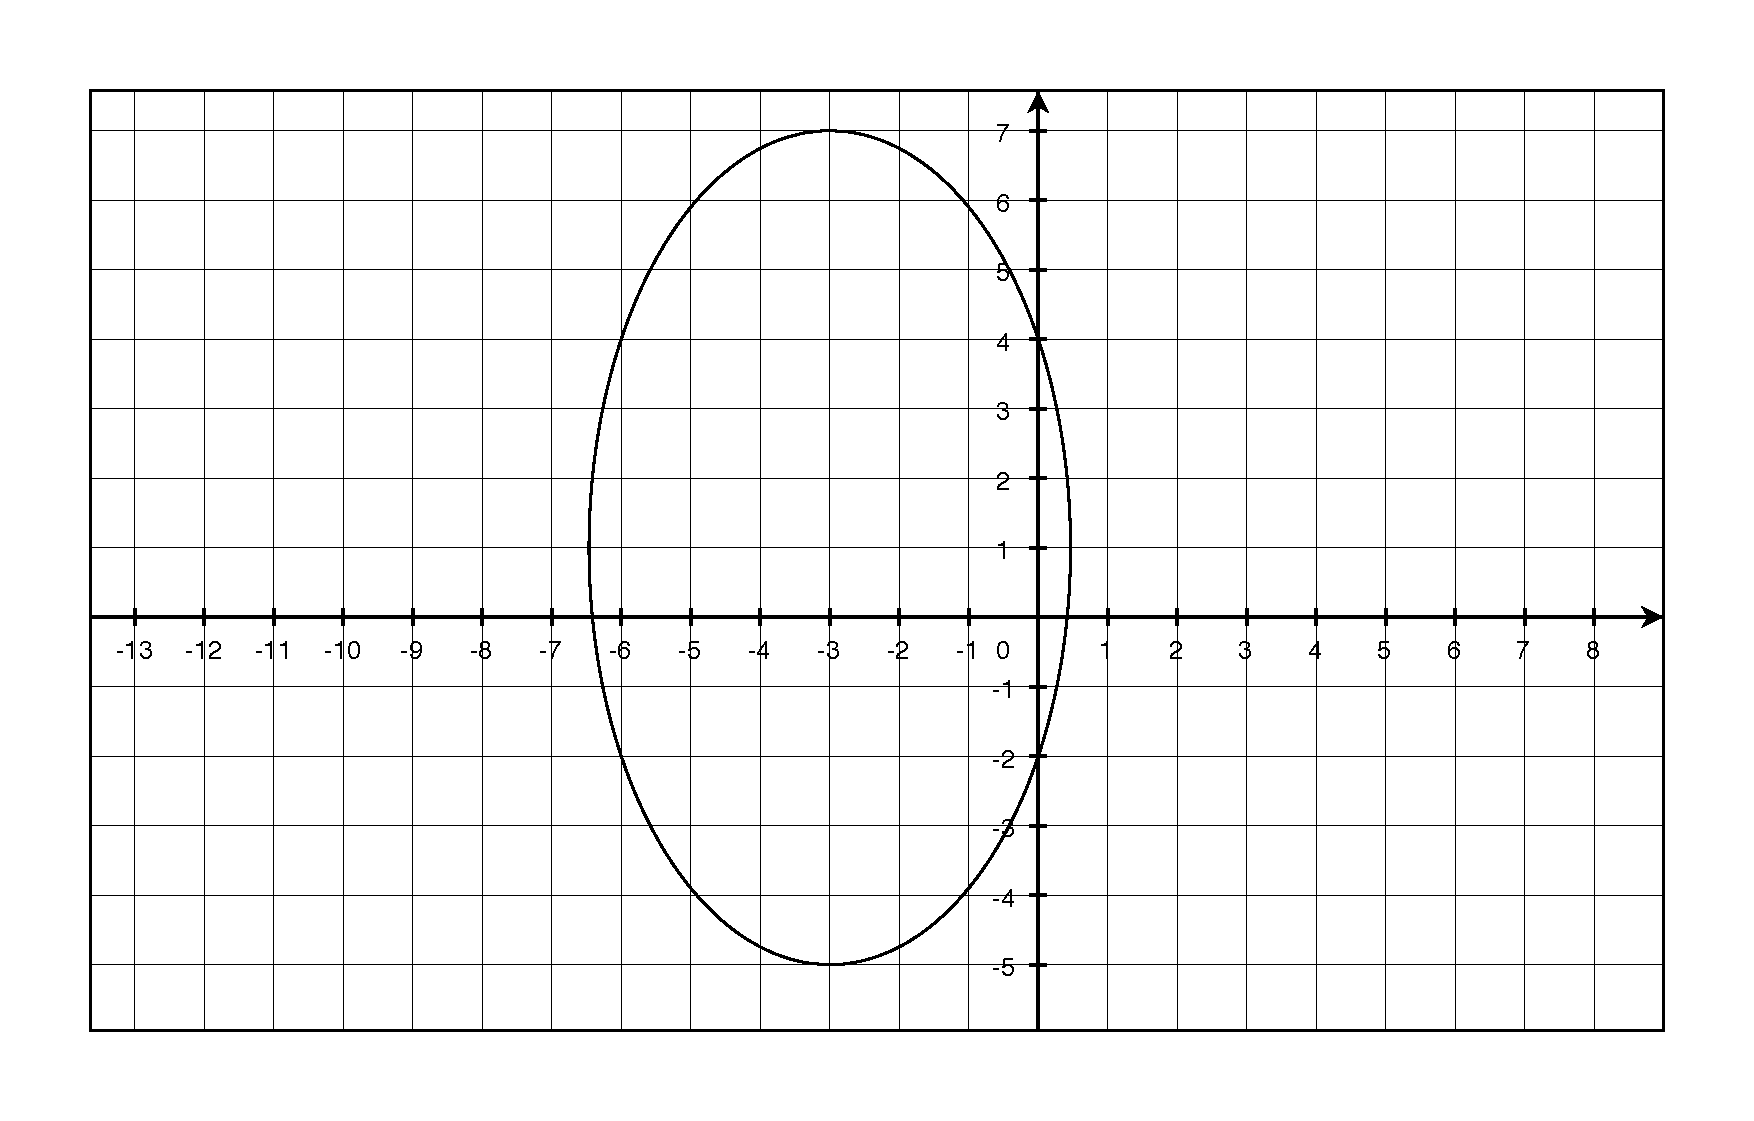
\includegraphics[scale=.3]{p792_18.eps}
  \caption*{Question 18}
\end{figure}

\item[19]
\begin{align*}
  6x^2 + 2y^2 + 18x - 10y + 2 &= 0 \\
  6(x^2 + 3x + \frac{9}{4}) + 2(y^2 - 5y + \frac{25}{4}) &= 24 \\
  \frac{(x+3/2)^2}{4} + \frac{(y-5/2)^2}{12} &= 1 \\
\end{align*}

\begin{tabular}{cccc}
\toprule
center & vertices & foci & eccentricity \\
\midrule
  $(-\dfrac{3}{2}, \dfrac{5}{2})$ & $(-\dfrac{3}{2}, \dfrac{5}{2} \pm 2 \sqrt{3})$ & $(-\dfrac{3}{2}, \dfrac{5}{2} \pm 2\sqrt{2})$ & $\dfrac{\sqrt{6}}{3}$ \\
\bottomrule
\end{tabular}

\begin{figure}[H]
  \centering
  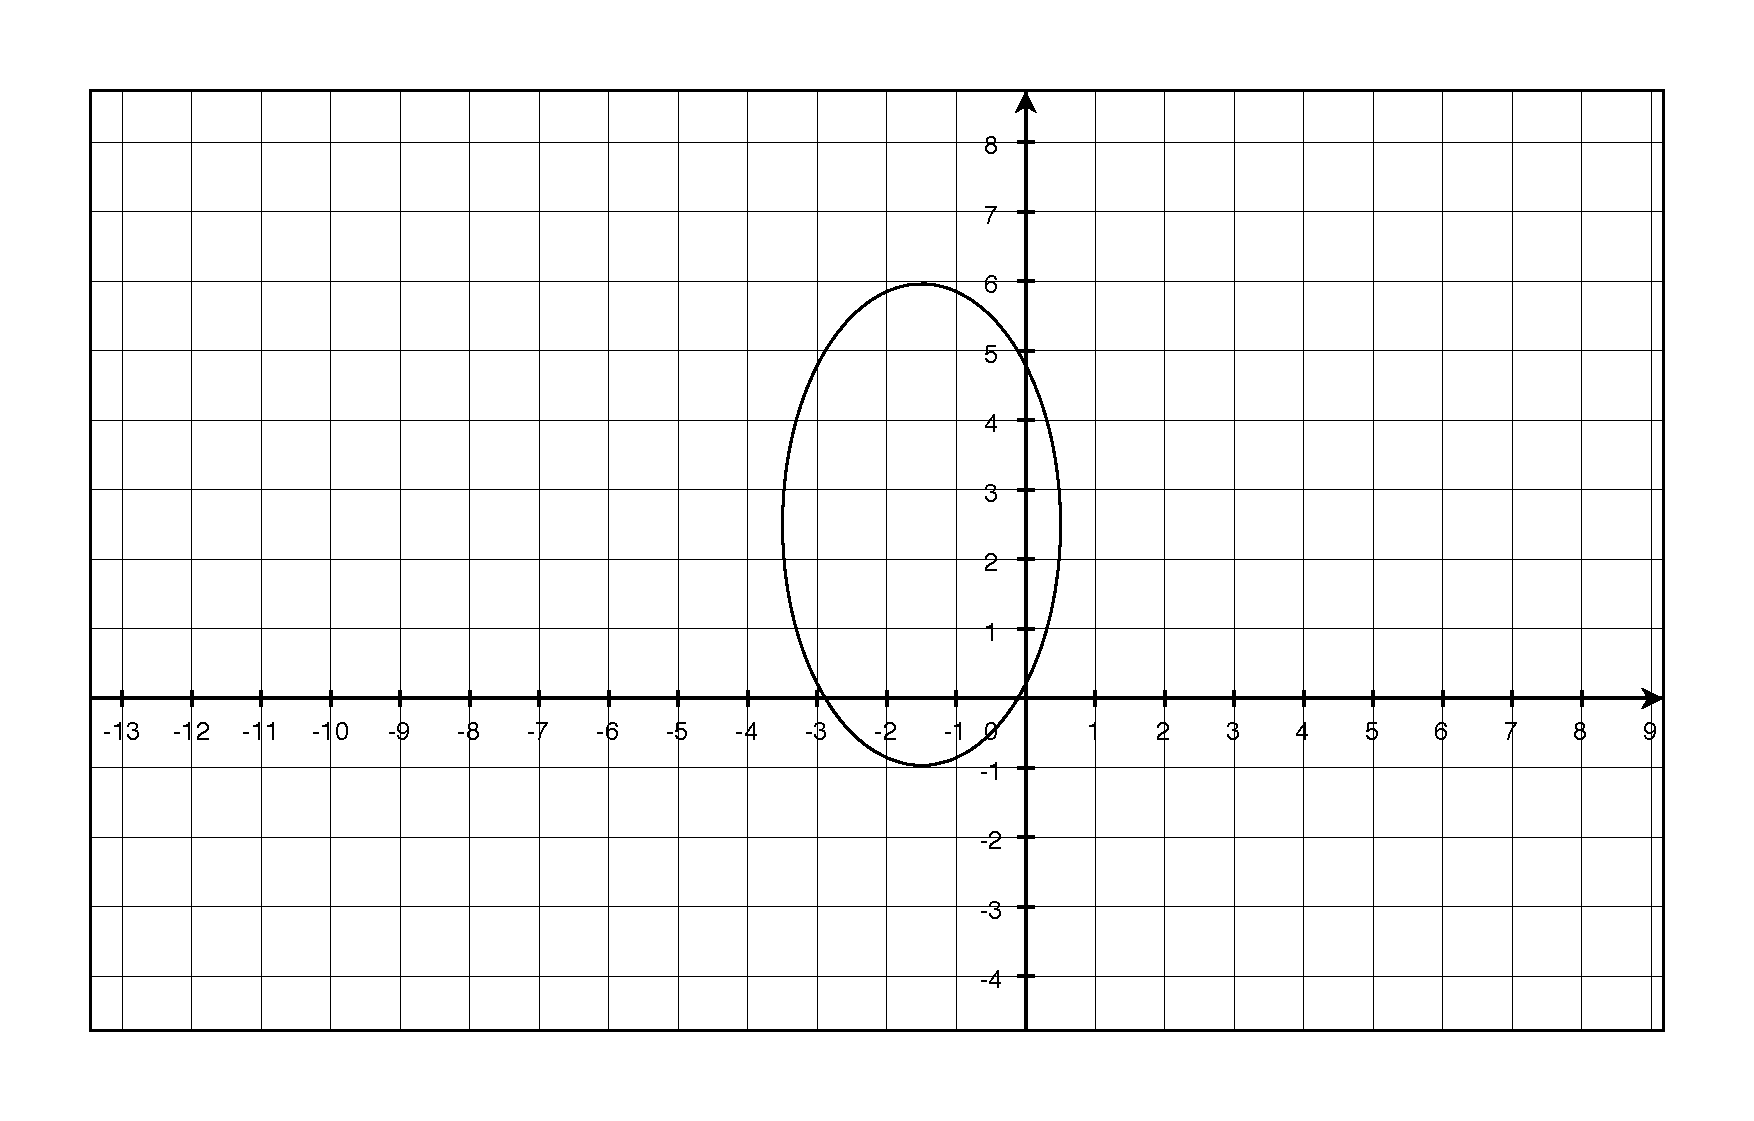
\includegraphics[scale=.3]{p792_19.eps}
  \caption*{Question 19}
\end{figure}

\item[27]
\begin{align*}
  a &= 4 \\
  b &= 2 \\
\end{align*}

equation:
\[
  \frac{x^2}{4} + \frac{y^2}{16} = 1
\]

% \item[28]
% \begin{align*}
%   a &= 2 \\
%   b &= \frac{3}{2} \\
% \end{align*}

% equation:
% \[
%   \frac{x^2}{4} + \frac{4 y^2}{9} = 1
% \]

\item[29]
\begin{align*}
  a &= 6 \\
  c &= 2 \\
  b^2 &= 6^2 - 2^2 = 32 \\
\end{align*}

equation:
\[
  \frac{x^2}{36} + \frac{y^2}{32} = 1
\]

% \item[30]
% \begin{align*}
%   a &= 8 \\
%   c &= 4 \\
%   b^2 &= 8^2 - 4^2 = 48 \\
% \end{align*}

% equation:
% \[
%   \frac{x^2}{48} + \frac{y^2}{64} = 1
% \]

\item[31]
\begin{align*}
  a &= 6 \\
  c &= 5 \\
  b^2 &= 6^2 - 5^2 = 11 \\
\end{align*}

equation:
\[
  \frac{x^2}{36} + \frac{y^2}{11} = 1
\]

\item[33]
\begin{align*}
  \frac{x^2}{b^2} + \frac{y^2}{25}  &= 1 \\
  \frac{4}{25} + \frac{16}{b^2} &= 1 \\
  b^2 &= \frac{400}{21} \\
\end{align*}

equation:
\[
  \frac{21 x^2}{400} + \frac{y^2}{25} = 1
\]


\item[34]
\begin{align*}
  \frac{0}{b^2} + \frac{16}{a^2}  &= 1 \\
  a^2 &= 16 \\
  \\
  \frac{4}{b^2} + \frac{0}{a^2}  &= 1 \\
  b^2 &= 4 \\
\end{align*}

equation:
\[
  \frac{x^2}{4} + \frac{y^2}{16} = 1
\]

\item[41]
\begin{align*}
  a &= 8 \\
  c &= 4 \\
  b^2 &= 8^2 - 16^2 = 48 \\
\end{align*}

center: $(0, 4)$

equation:
\[
  \frac{x^2}{48} + \frac{(y-4)^2}{64} = 1
\]

\item[43]

\begin{align*}
  a &= 4 \\
  b &= 3 \\
\end{align*}

center: $(3, 5)$

equation:
\[
  \frac{(x-3)^2}{9} + \frac{(y-5)^2}{16} = 1
\]

\item[47]

\begin{align*}
  a &= 5 \\
  c &= 3 \\
  b^2 &= 5^2 - 3^2 = 16 \\
\end{align*}

center: $(0, 0)$

equation:
\[
  \frac{x^2}{25} + \frac{y^2}{16} = 1
\]

\item[51]
\begin{align*}
  \pi ab &= 2 \pi b^2 \\
  a &= 2b = 2 \cdot 10 = 20 \\
\end{align*}

The length of the major axis is 40.

\item[52]
\begin{align*}
  a &= \frac{36.18}{2} = 18.09 \\
  \\
  \frac{c}{a} &= 0.97 \\
  c &= 0.97 \cdot 18.09 =  17.55 \\
  \\
  b^2 &= 18.09^2 - 17.55^2 = 19.25
\end{align*}

equation:
\[
  \frac{x^2}{327.25} + \frac{y^2}{19.25} = 1
\]

\section{Pages 802-803}

\item[1]
b

\item[2]
c

\item[3]
a

\item[4]
d

\item[7]
\[
  \frac{y^2}{25} - \frac{x^2}{81} = 1
\]

\begin{tabular}{ccc}
\toprule
center & vertices & foci \\
\midrule
  $(0, 0)$ & $(0, \pm 5)$ & $(\pm \sqrt{106}, 0)$ \\
\bottomrule
\end{tabular}

\begin{figure}[H]
  \centering
  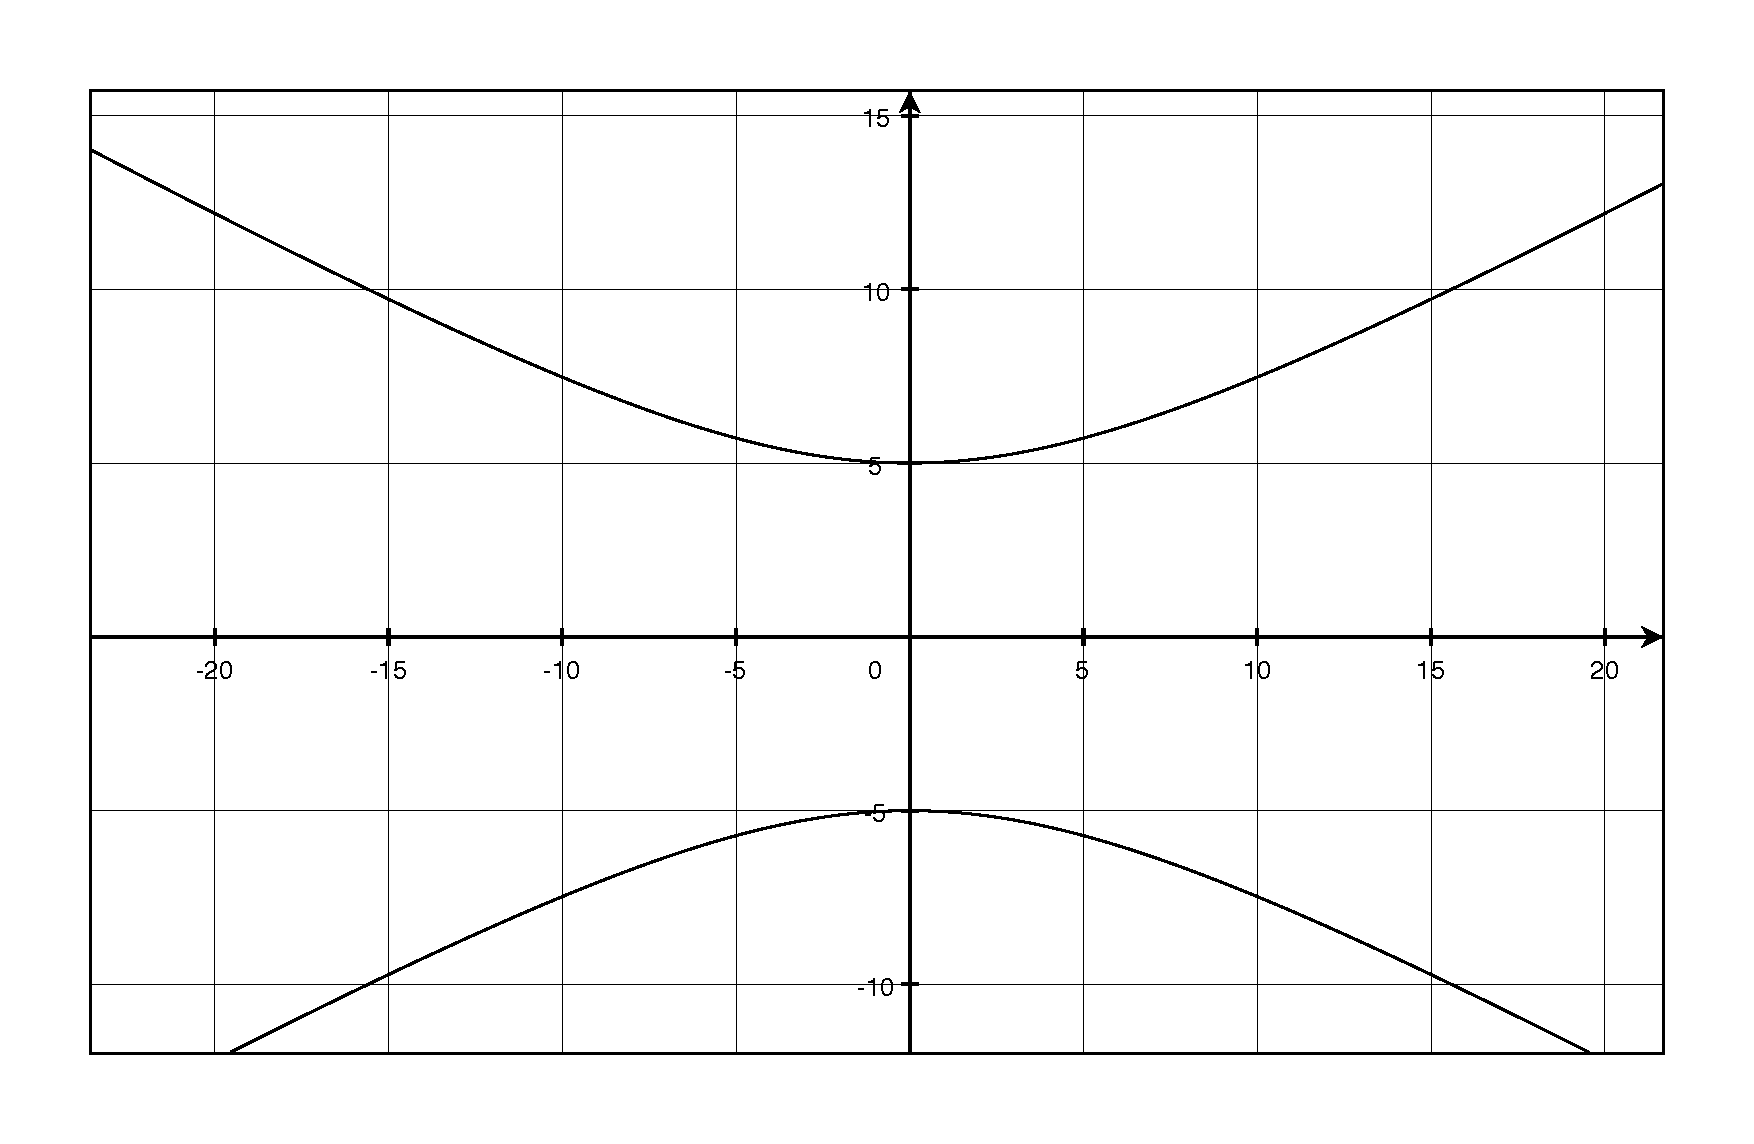
\includegraphics[scale=.3]{p802_7.eps}
  \caption*{Question 7}
\end{figure}

\item[8]
\[
  \frac{x^2}{36} - \frac{y^2}{4} = 1
\]

\begin{tabular}{ccc}
\toprule
center & vertices & foci \\
\midrule
  $(0, 0)$ & $(\pm 6, 0)$ & $(0, \pm 4 \sqrt{2})$ \\
\bottomrule
\end{tabular}

\begin{figure}[H]
  \centering
  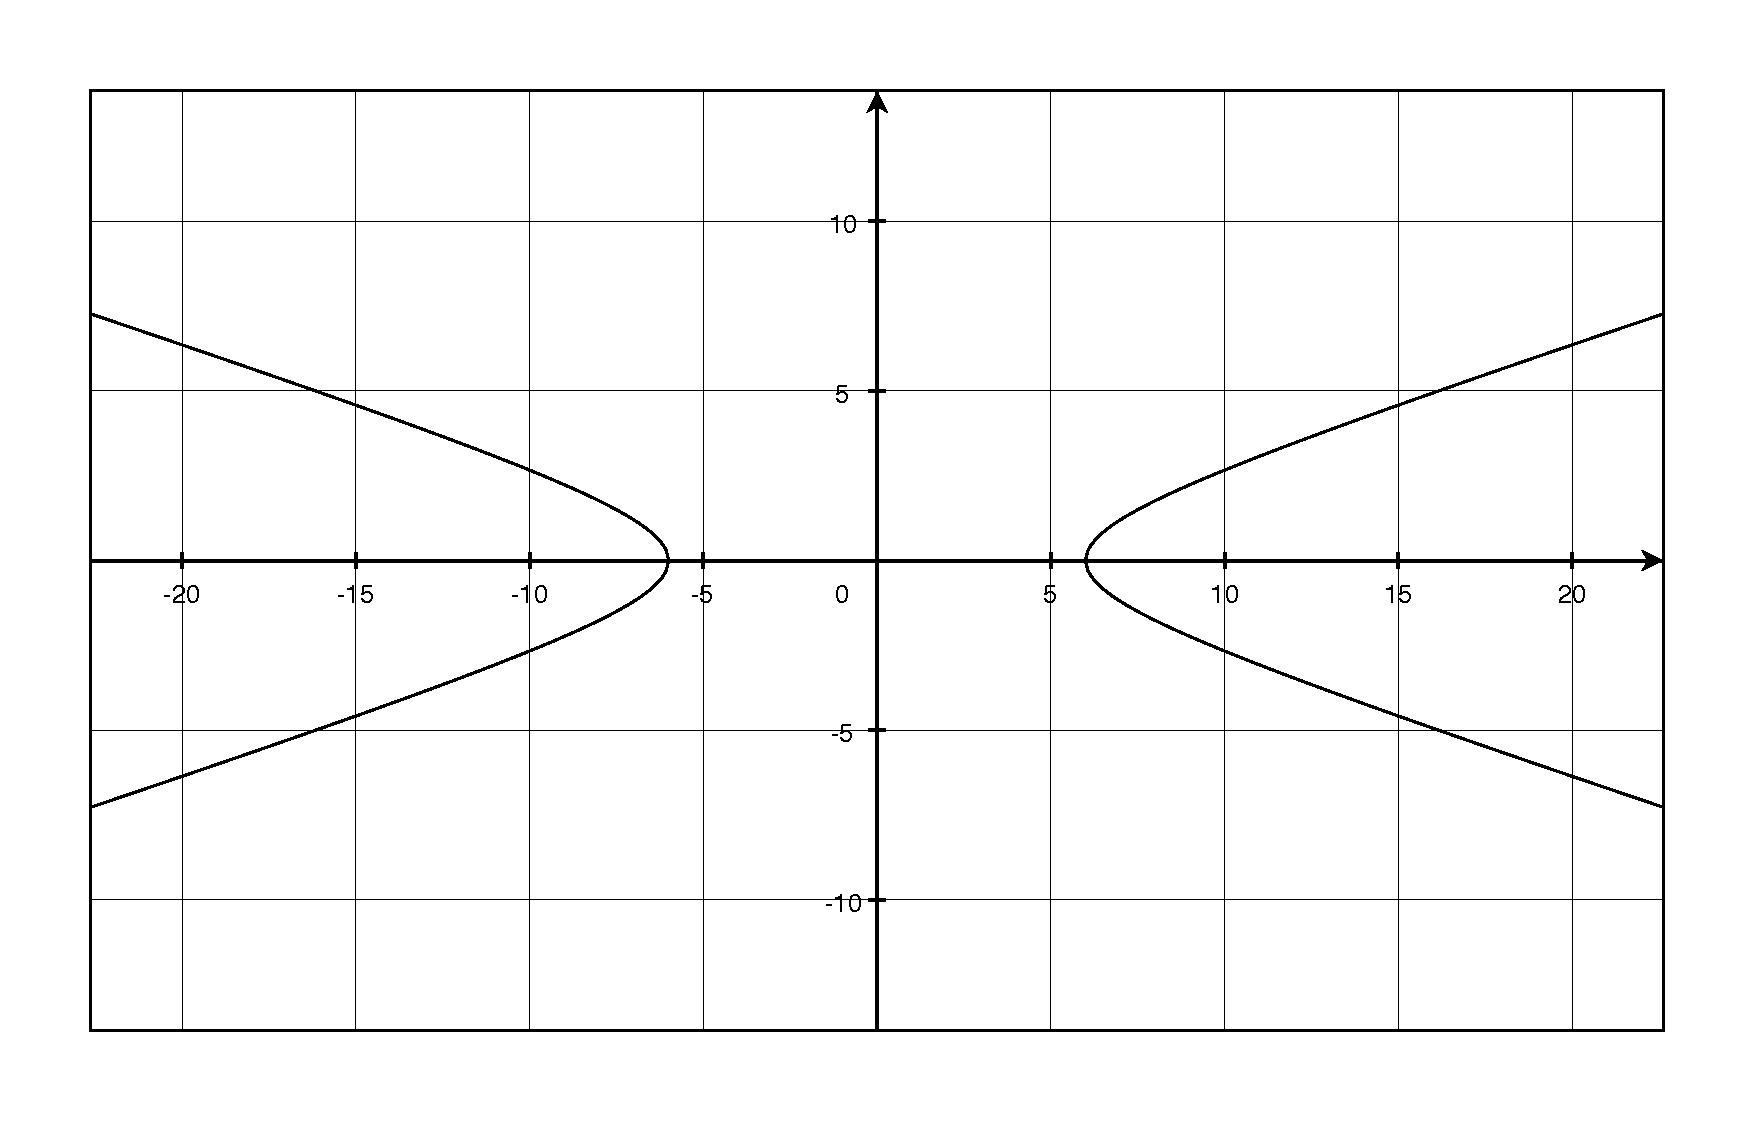
\includegraphics[scale=.3]{p802_8.eps}
  \caption*{Question 8}
\end{figure}

\item[9]
\[
  \frac{(x-1)^2}{4} - \frac{(y+2)^2}{1} = 1
\]

\begin{tabular}{cccc}
\toprule
center & vertices & foci & asymptotes \\
\midrule
  $(1, -2)$ & $(-1, -2)$, $(3, -2)$ & $(1 \pm \sqrt{5}, -2)$ & $-2 \pm \dfrac{1}{2}(x-1)$ \\
\bottomrule
\end{tabular}

\begin{figure}[H]
  \centering
  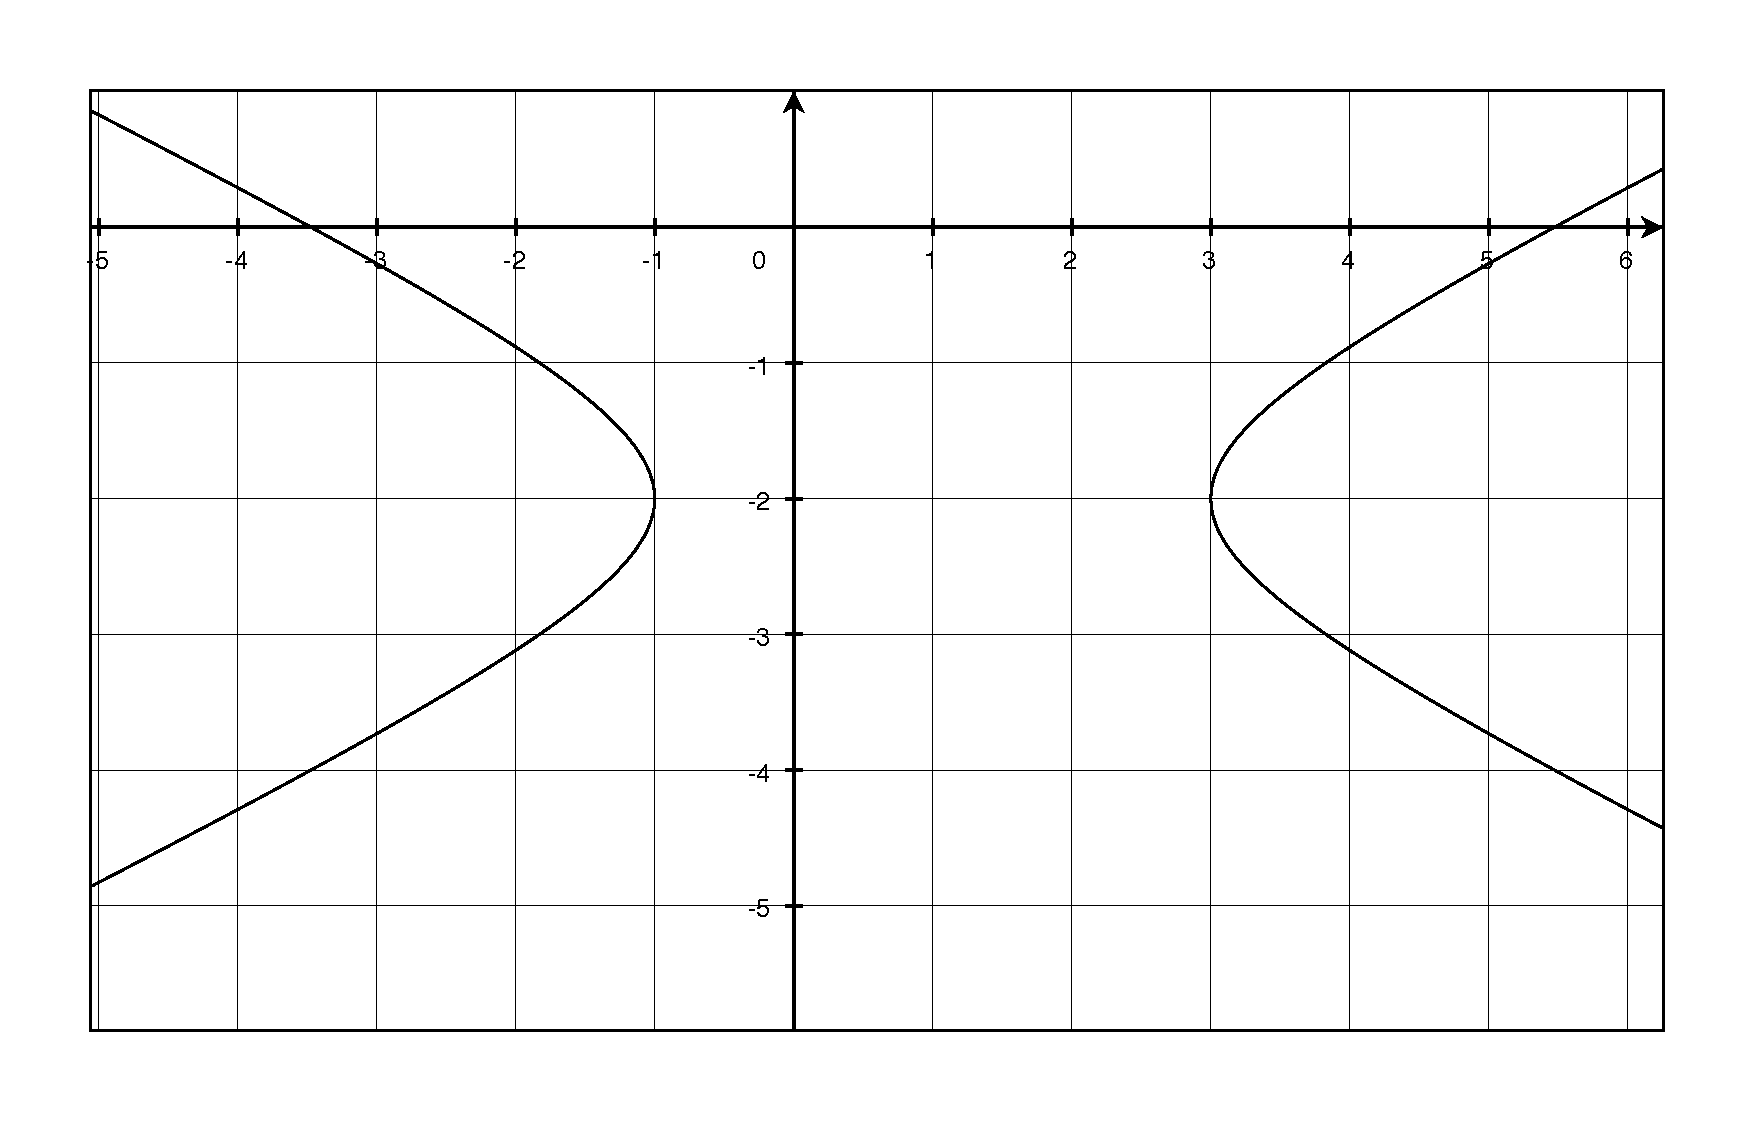
\includegraphics[scale=.3]{p802_9.eps}
  \caption*{Question 9}
\end{figure}

\item[10]
\[
  \frac{(x+3)^2}{144} - \frac{(y-2)^2}{25} = 1
\]

\begin{tabular}{ccc}
\toprule
center & vertices & foci \\
\midrule
  $(-3, 2)$ & $(-15, 2)$, $(9, 2)$ & $(-16, 2)$, $(10, 2)$ \\
\bottomrule
\end{tabular}

\begin{figure}[H]
  \centering
  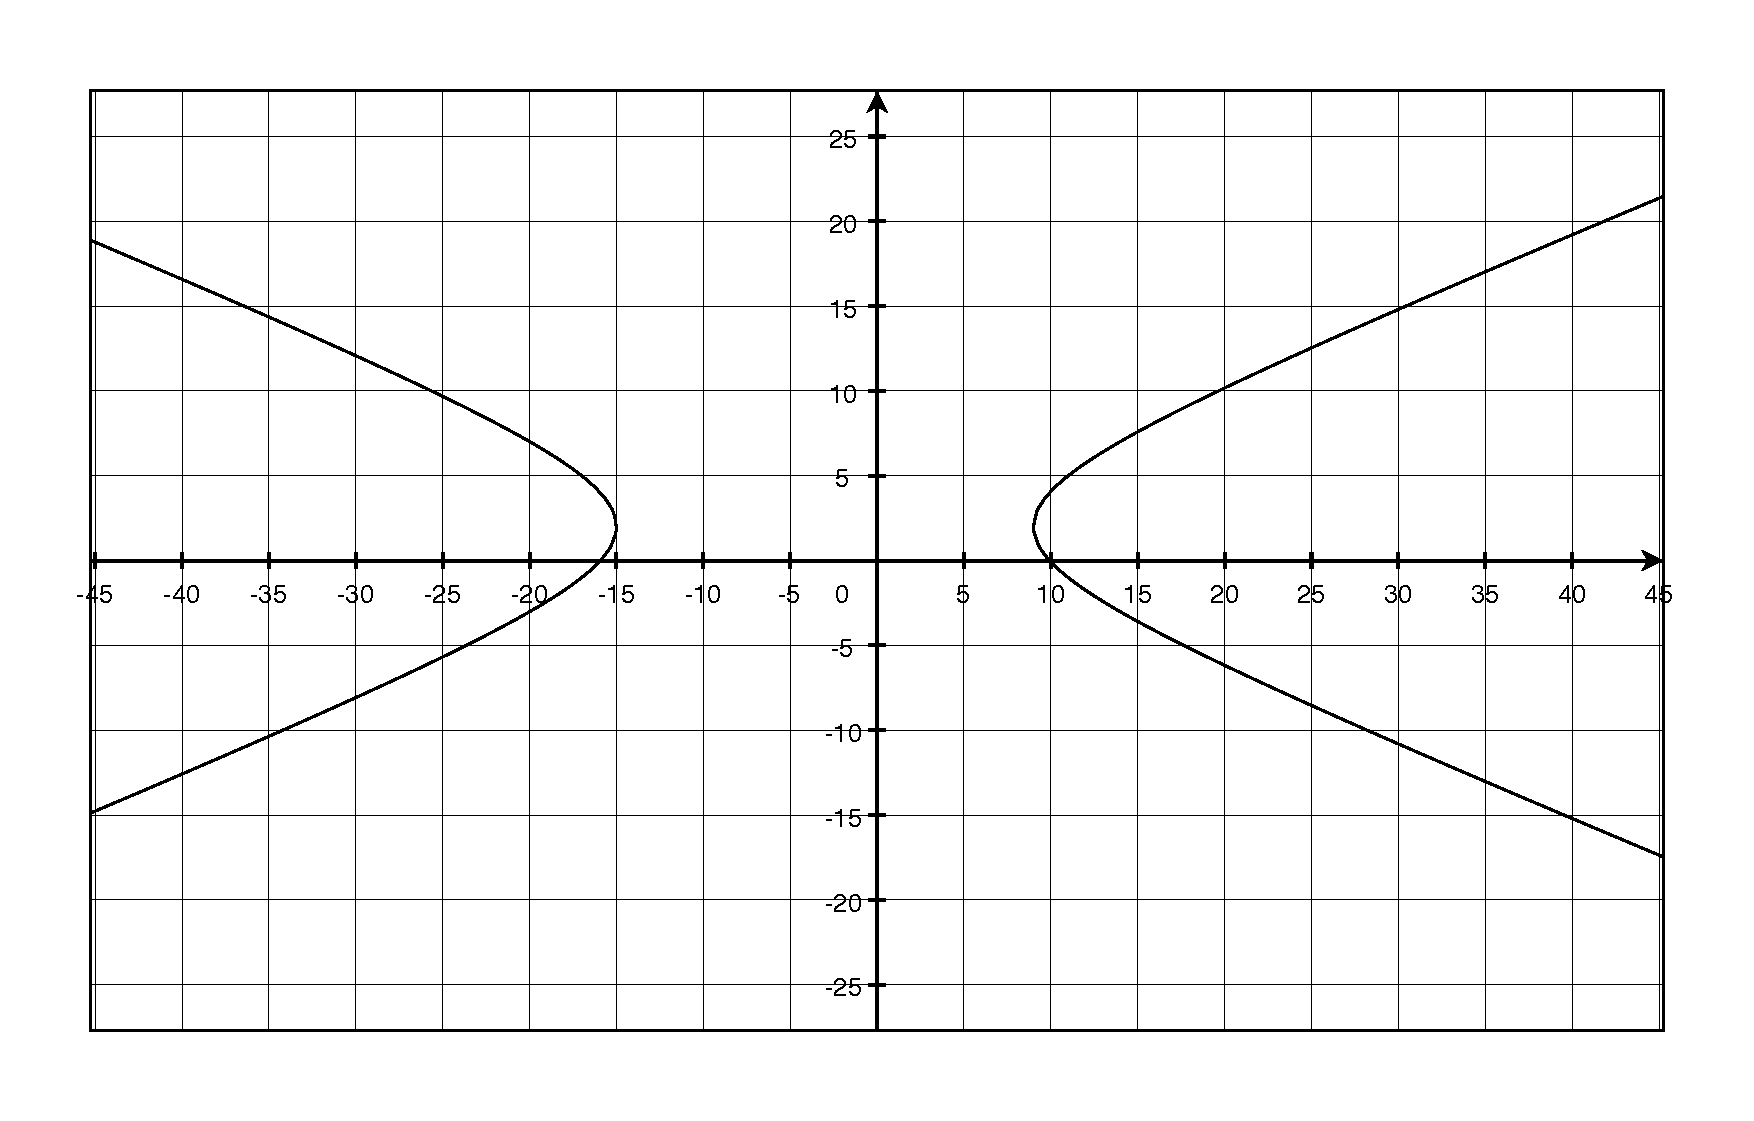
\includegraphics[scale=.3]{p802_10.eps}
  \caption*{Question 10}
\end{figure}

\item[21]
\begin{itemize}
  \item vertices: $(0, \pm 2)$
  \item foci: $(0, \pm 4)$
\end{itemize}

\begin{align*}
  a &= 2 \\
  c &= 4 \\
  b^2 &= 4^2 - 2^2 = 12 \\
\end{align*}

center: $(0, 0)$

\[
  \frac{y^2}{4} - \frac{x^2}{12} = 1 
\]

\item[23]
\begin{itemize}
  \item vertices: $(\pm 1, 0)$
  \item asymptotes: $y = \pm 5x$
\end{itemize}

\begin{align*}
  a &= 1 \\
  b &= 5 \\
\end{align*}

center: $(0, 0)$

\[
  \frac{x^2}{1} - \frac{y^2}{25} = 1 
\]

\item[25]

\begin{itemize}
  \item foci: $(0, \pm 8)$
  \item asymptotes: $y = \pm 4x$
\end{itemize}


\begin{align*}
  a &= 4b \\
  \\
  a^2 + b^2 &= 8^2 \\
  (4b)^2 + b^2 &= 64 \\
  17b^2 &= 64 \\ 
  b^2 &= \frac{64}{17} \\ 
  \\
  a^2 &= 64 - \frac{64}{17} = \frac{1024}{17} \\ 
\end{align*}

center: $(0, 0)$

\[
  \frac{17 y^2}{1024} - \frac{17x^2}{64} = 1 
\]

\item[27]

\begin{itemize}
  \item vertices: $(2, 0)$, $(6, 0)$
  \item foci: $(0, 0)$, $(8, 0)$
\end{itemize}

center: $(4, 0)$

\begin{align*}
  a &= 2 \\
  c &= 4 \\
  b^2 &= 4^2 - 2^2 = 12 \\
\end{align*}

\[
  \frac{(x-4)^2}{4} - \frac{y^2}{12} = 1 
\]

\item[42]
ellipse

\item[43]
ellipse

\item[44]
hyperbola

\item[45]
parabola

\item[46]
ellipse

\item[47]
hyperbola

\item[48]
parabola

\item[49]
circle

\end{description}

\else

\vspace{4 in}

% \begin{em}
%   Under a government which imprisons any unjustly, the true place for a just man is also a prison. The proper place
%   to-day, the only place which Massachusetts has provided for her freer and less desponding spirits, is in her prisons,
%   to be put out and locked out of the State by her own act, as they have already put themselves out by their
%   principles. It is there that the fugitive slave, and the Mexican prisoner on parole, and the Indian come to plead the
%   wrongs of his race, should find them; on that separate, but more free and honorable ground, where the State places
%   those who are not with her, but against her — the only house in a slave State in which a free man can abide with honor.
% \end{em}

% \vspace{.2 cm}
% \hspace{1.5 cm} --Henry David Thoreau, {\em Civil Disobedience}

\begin{em}
  Good pitching will always stop good hitting, and vice versa.
\end{em}

\vspace{.2 cm}
\hspace{1.5 cm} --Casey Stengel

\fi

\end{document}

